%%%
%%% OpenCAEシンポジウムTeXテンプレートファイル
%%% template_OpenCAE_symposium.tex
%%% OpenCAEシンポジウム2018版
%%%
%%
%% ltjocはOpenCAE論文集・シンポジウム用のクラスファイルです.変更しないでください.
%% 本文が英語の場合には,オプションにenglishを指定してください.
\documentclass{../../style/ltjoc}
%\documentclass[english]{../../style/ltjoc}
%%
%% 表題(title),副題(subtitle),著者(author),所属(affiliation)
%% 本文が英語の場合には,こちらに英文表題,英文副題,英文著者,英文所属を記述します.
\title{GetFEM++ ユーザドキュメントの地域化L10N}
% 副題が無い場合にはコメントアウトします.
\subtitle{日本語翻訳作業} 
\author{%
\href{https://twitter.com/tkoyama010}{@tkoyama010}$^{1\dagger}$%
}
\affiliation{%
${}^{1}$\href{https://tkoyama010.github.io/getfem-docs-html-ja/}{GetFEM++ Japanese Team}%
} 
%%
%% Corresponding authorの電子メールアドレス
%% 本論文について連絡が取れる著者の電子メールアドレスを記載してください.
\AuthorsEmail{tkoyama010@gmail.com}
%%
%% 英文表題(etitle),英文副題(esubtitle),英文著者(eauthor),英文所属(eaffiliation)
%% 本文が英語の場合には表示されません.
\etitle{Localization(L10N) of GetFEM++ User Document}
% 副題が無い場合にはコメントアウトします.
\esubtitle{Translation for Japanese}
\eauthor{%
\href{https://twitter.com/tkoyama010}{@tkoyama010}$^{*\dagger}$%
}
\eaffiliation{%
${}^{*}$\href{https://tkoyama010.github.io/getfem-docs-html-ja/}{GetFEM++ Japanese Team}%
}
%%
%% キーワード
\keywords{GetFEM++, L10N, Sphinx, Transifex, translate-shell}
%%
%% 英文概要
%% 英文概要を省略する場合には,abstract環境の定義をしないでください.
\begin{abstract}
The GetFEM++ project focuses on the development of a generic and efficient C++ library for finite element methods elementary computations.
The document of this library are generated by Sphinx and are available for modification and reuse under the terms of the GNU Free Documentation License .
So, we translated this document to Japanese by using Transifex and distributed it in TechBookFest5.
\end{abstract}
%%
%% luatexja-fontspecパッケージ
\usepackage{luatexja-fontspec}
\defaultfontfeatures{Ligatures=TeX}
%% luatexja-presetパッケージ
%% 和文フォントのプリセット設定
%% オプションにnoembed(非埋込)を指定しないでください.
%\usepackage[ipaex]{luatexja-preset} % IPAex(デフォルト)
%\usepackage[ms]{luatexja-preset} % MS
%\usepackage[hiragino-pro]{luatexja-preset} % ヒラギノPro
%%
%% 欧文フォントの指定
%% 使用できるフォントについては,以下のコマンドで調べてください.
%% $ luaotfload-tool --list=*
%%
%% 欧文通常フォント
%\setmainfont{Cambria} % Cambria
%\setmainfont{Times New Roman} % Times New Roman
%\setmainfont{TeXGyreTermes} % TeXGyreTermes
%%
%% 欧文Sans-serifフォント
%\setsansfont{Calibri} % Calibri
%\setsansfont{Arial} % Arial
%\setsansfont{Helvetica} % Helvetica
%\setsansfont{TeXGyreHeros} % TeXGyreHeros
%%
%% 欧文monospaceフォント
%\setmonofont{Consolas} % Consolas
%\setmonofont{Courier New} % Courier New
%\setmonofont{Lucida Console} % Lucida Console
%%
%% subfigureパッケージ
\usepackage{subfigure}
%%
%% graphicxパッケージ
\usepackage{graphicx}
%% color パッケージ
\usepackage[usenames]{color}
%%
%% shdocパッケージ
\usepackage[
 backgroundcolor=gray!50,
 usernamecolor=black,
 machinenamecolor=black,
 indicatorcolor=black,
 separatorcolor=black,
 pathcolor=black,
 optioncolor=black,
 textcolor=black
]{shdoc}
%%
%% underscoreパッケージ
\usepackage{underscore}
%%
%% draftwatermarkパッケージ
\usepackage{draftwatermark}
%% listingsパッケージ
\usepackage{listings}
\lstset{
  basicstyle = \ttfamily,
  frame=single,
  tabsize=2,
  breaklines=true
}
\lstdefinelanguage{diff}{
  morecomment=[f][\color{blue}]{@@},     % group identifier
  morecomment=[f][\color{red}]-,         % deleted lines 
  morecomment=[f][\color{OliveGreen}]+,  % added lines
  morecomment=[f][\color{magenta}]{---},   % Diff header lines (must appear after +,-)
  morecomment=[f][\color{magenta}]{+++},
}
%%
%% hyperrefパッケージ
\usepackage[
 pdfencoding=auto,
 bookmarks=true,
 bookmarksnumbered=true,
 colorlinks=true,
 allcolors={blue}
]{hyperref}
%%
%% autorefでの図表の参照名の再定義
\makeatletter
\if@english
  \renewcommand*{\figureautorefname}{\figurename}
  \renewcommand*{\tableautorefname}{\tablename}
\else
  \renewcommand*{\figureautorefname}{図}
  \renewcommand*{\tableautorefname}{表}
\fi
\makeatother
%%
%% ヘッダ右の設定
%% シンポジウム毎に決められています.変更しないでください.
\markright{OpenCAE Symposium 2018, Dec. 8-9, 2018, Kawasaki} % Do not edit this line
%%
%% 本文
\begin{document}
%%
%% 題目などの出力
\maketitle
%%%
\section{はじめに}
\href{http://getfem.org}{GetFEM++}は汎用的で効率的な有限要素法の\href{https://isocpp.org/}{C++}ライブラリです。
有限要素法を用いて線形および非線形偏微分方程式を解くためのフレームワークを提供することを目指しています。
\href{http://getfem.org}{GetFEM++}ライブラリには多くの文書があり、その多くはさまざまな著者によって寄稿されています。
\href{http://getfem.org}{GetFEM++}の文書化に使用されるマークアップは\href{http://docutils.sourceforge.net/}{docutils}プロジェクトによって
開発された\href{http://docutils.sourceforge.net/rst.html}{reStructuredText}で、
\href{http://www.sphinx-doc.org/ja/stable/}{Sphinx}というツールセットを使用しています。
また、ドキュメントは\href{https://www.gnu.org/licenses/fdl.html}{GNU Free Documentation License}により改変および頒布が許可されています。

そこで、\href{http://www.sphinx-doc.org/ja/stable/}{Sphinx}の国際化機能を使用して\href{http://getfem.org}{GetFEM++}のドキュメント翻訳作業を
翻訳プラットホーム\href{https://www.transifex.com}{Transifex}で行いました。
さらに、技術同人誌即売会である\href{https://techbookfest.org/event/tbf05}{技術書典5}で翻訳したドキュメントの頒布を行いました。
本報告では翻訳作業の手順と頒布の活動について紹介します。
操作環境は\href{https://www.ubuntu.com/}{Ubuntu}18.04です。

\section{\href{http://getfem.org}{GetFEM++}プロジェクト}
\href{http://getfem.org}{GetFEM++}の英語の\href{https://en.wikipedia.org/wiki/GetFEM++}{Wikipedia}を翻訳し、
日本語の\href{https://ja.wikipedia.org/wiki/GetFEM++}{Wikipedia}を作成しました。
以下に内容を引用します。

\begin{quote}
GetFEM++ は Python, Matlab そして Scilabのインタフェースを使用可能なC++の汎用ライブラリである。
このライブラリの目的は有限要素法を用いて線形および非線形偏微分方程式を解くためのフレームワークを提供することである。
有限要素近似や数値積分法の選択の柔軟性が特徴の一つである。
\texttt{「\href{https://ja.wikipedia.org/wiki/GetFEM++}{GetFEM++ - Wikipedia}」(Oct.13,2018 12:01 UTC) より引用}
\end{quote}
ライセンスや受賞歴については\href{https://ja.wikipedia.org/wiki/GetFEM++}{ページ}を参照してください。
\href{http://www.getfem.org/tutorial/index.html}{GetFEM++のチュートリアル}には\autoref{fig:getfem-tutorial}に示す例が掲載されています。

\begin{figure}
%\centering
\subfigure[\href{http://www.getfem.org/tutorial/thermo_coupling.html}{熱弾性的および電気結合の例}]{
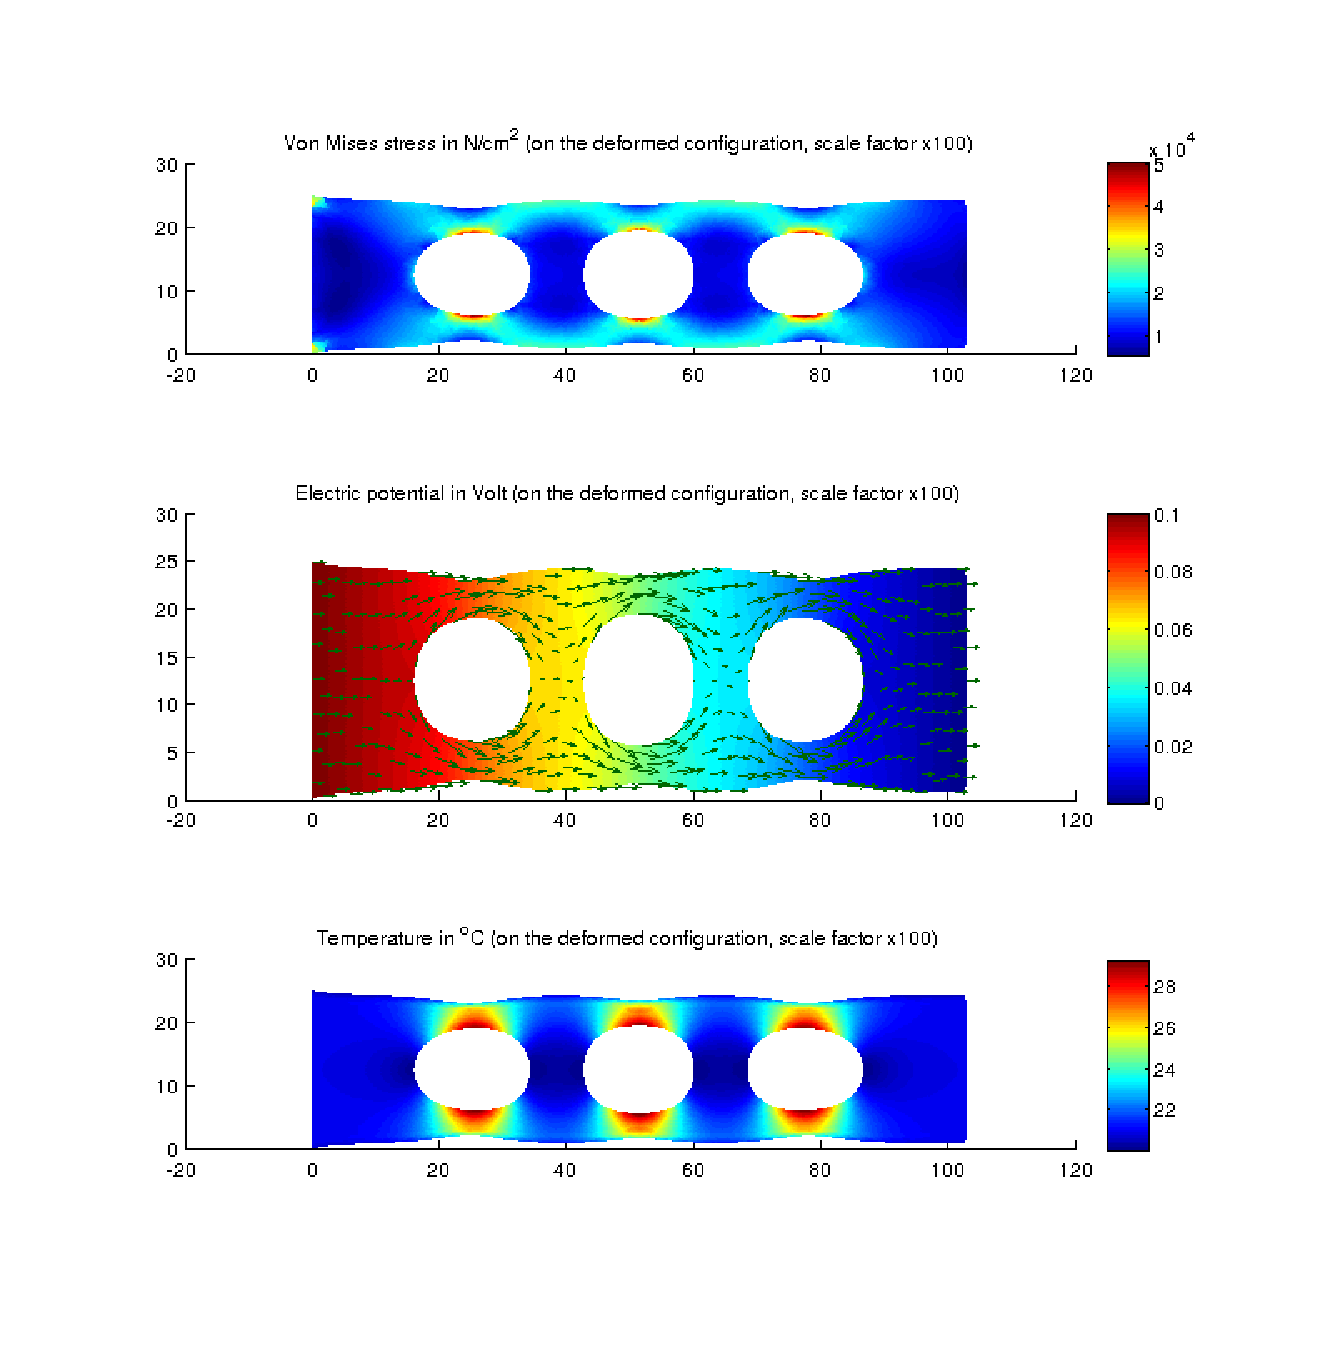
\includegraphics[width=0.50\textwidth]{fig/solution-thermo.eps}
}
\subfigure[\href{http://www.getfem.org/tutorial/wheel.html}{車輪の接触の例}]{
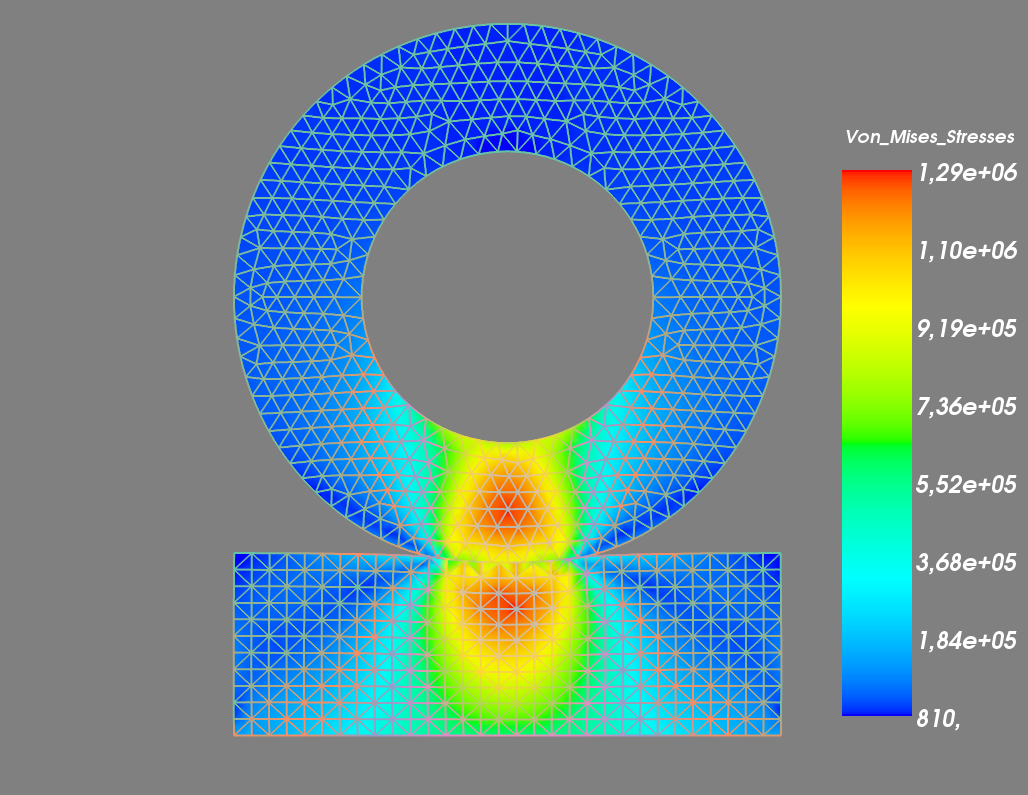
\includegraphics[width=0.45\textwidth]{fig/wheel.eps}
}
\caption{GetFEM++を使用した解析例}
\label{fig:getfem-tutorial}
\end{figure}

\href{http://getfem.org}{GetFEM++}はソースのホスティングサービスとして\href{https://savannah.gnu.org}{Savannah}を使用しています。
GNU \href{https://savannah.gnu.org}{Savannah}についてWikipediaの説明を引用します。
\begin{quote}
GNU Savannah は、フリーソフトウェアプロジェクトのための協働型ソフトウェア開発管理システムを提供するフリーソフトウェア財団のプロジェクトです。
現在は、CVS、GNU arch、Subversion、Git、Mercurial、GNU Bazaar、メーリングリスト、ウェブホスティング、ファイルホスティング、バグ管理サービスといった機能を提供しています。
Savannah は、SourceForge.netと同じソフトウェアをベースとしたホスティングサービスシステムである Savane を使っています。

\texttt{「\href{https://savannah.gnu.org}{GNU Savannah - Wikipedia}」(Oct.13,2018 11:31 UTC) より引用}
\end{quote}
このように、\href{https://savannah.gnu.org}{Savannah}はGNUプロジェクトやフリーソフトのホスティングサービスとして広く使われています。
このホスティングサービスでは非開発ユーザの場合、以下のようにして、リポジトリをクローンします。
\begin{shbox}
  \shuser{user}
  \shline{}{git clone https://git.savannah.nongnu.org/git/getfem.git}
\end{shbox}
また、ソースからコンパイルする必要のない場合には以下のように\texttt{aptitude}(もしくは\texttt{apt})コマンドによりインストールすることも可能です。
\begin{shbox}
  \shuser{user}
  \shline{}{sudo aptitude install python-getfem++ libgetfem++-dev}
\end{shbox}
これにより\href{http://getfem.org}{GetFEM++}の\href{https://www.python.org/}{Python}インターフェースとライブラリがインストールされます。

一方、Savannahのプロジェクトの開発に参加するには\autoref{fig:savannah-new-user}の"New User"からユーザー登録が必要です。
\begin{figure}[htbp]
\centering
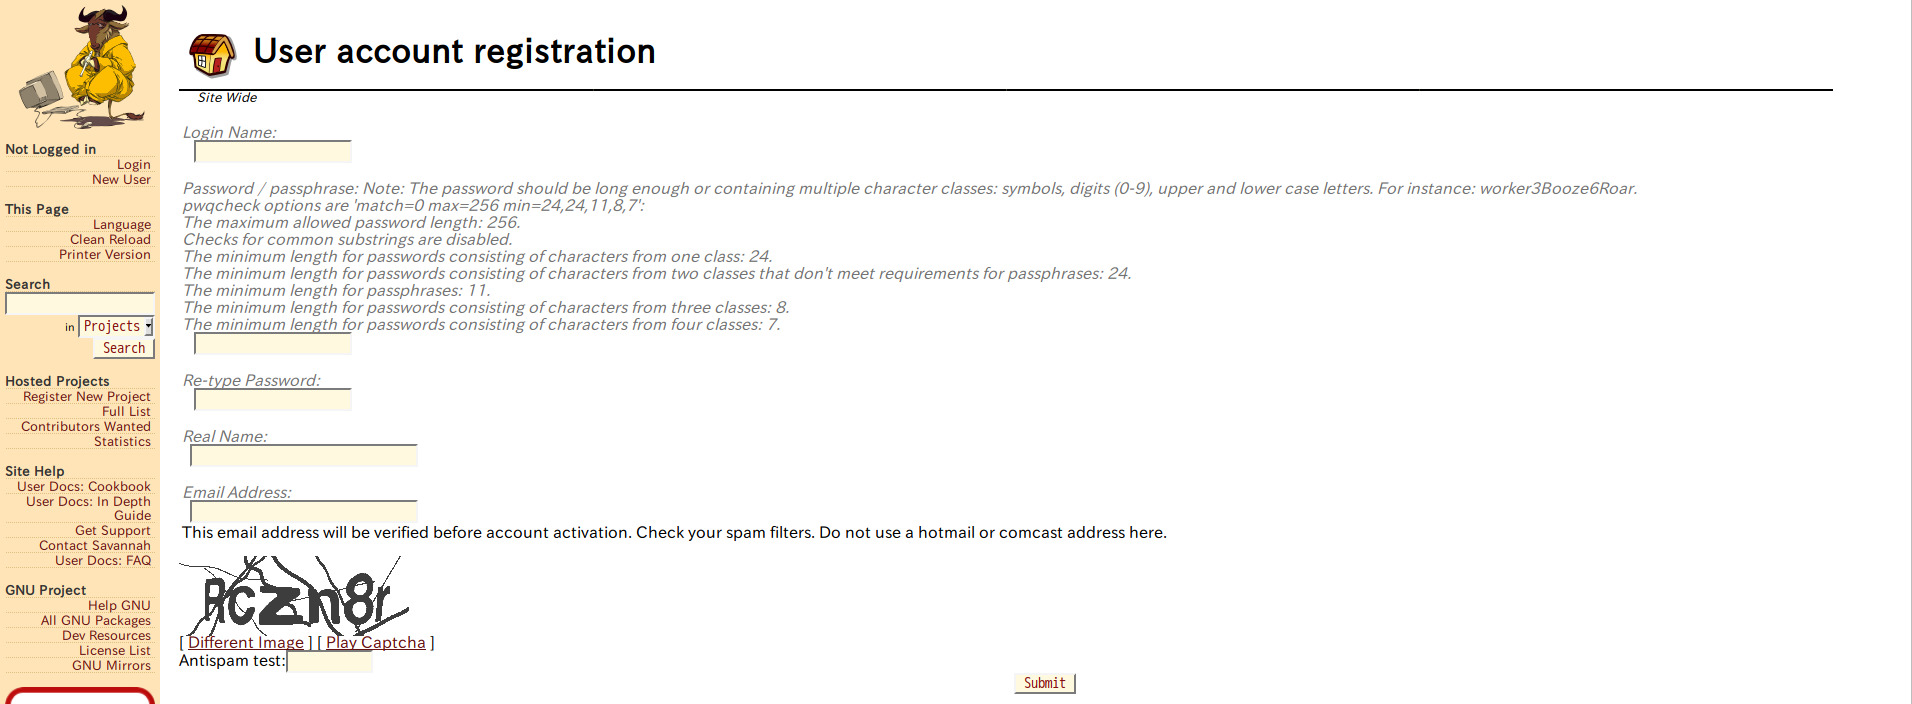
\includegraphics[width=1.0\textwidth]{fig/savannah-new-user.eps}
\caption{\href{https://savannah.gnu.org/account/register.php}{Savannahの新規ユーザ作成画面}}
\label{fig:savannah-new-user}
\end{figure}
開発者としてプロジェクトに参加するには、管理者にメッセージを送信し参加を承認してもらう必要があります。
2018年10月現在の\href{http://getfem.org}{GetFEM++}の管理者は \href{http://www.dtu.dk/english/service/phonebook/person?id=65472&tab=2&qt=dtupublicationquery}{Konstantinos Poulios} 氏と \href{http://math.univ-lyon1.fr/~renard/}{Yves Renard} 氏です。
開発者として権限が与えられたら、\href{http://getfem.org/project/index.html}{How to contribute / Git repository on Savannah}を参考にプロジェクトにコミットをします。
開発者として、リポジトリをクローンする場合は以下のようにします。
\begin{shbox}
  \shuser{developer}
  \shline{}{git clone ssh://savannah-login@git.sv.gnu.org:/srv/git/getfem.git}
\end{shbox}
ここで、\texttt{savannah-login}はSavannahに登録したユーザ名です。
ただし、何の設定もせずこれを実行すると認証エラーが発生します。
このコマンドを実行する前にSavannahに認証鍵を登録しておく必要があります。
まずは、ホームディレクトリで\texttt{ssh-keygen}コマンドを実行して認証鍵を作成してください。
\begin{shbox}
  \shuser{developer}
  \shline{}{cd /home/developer}
  \shline{}{ssh-keygen}
  \shoutput{}{Generating public/private rsa key pair.}
  \shoutput{}{Enter file in which to save the key (/home/developer/.ssh/id\textunderscore{}rsa):}
  \shoutput{}{Created directory '/home/developer/.ssh'.}
  \shoutput{}{Enter passphrase (empty for no passphrase):}
  \shoutput{}{Enter same passphrase again:}
  \shoutput{}{Your identification has been saved in /home/developer/.ssh/id\textunderscore{}rsa.}
  \shoutput{}{Your public key has been saved in /home/developer/.ssh/id\textunderscore{}rsa.pub.}
  \shoutput{}{The key fingerprint is:}
  \shoutput{}{SHA256:NVKmqK8YvqZiSakm3NO5+zLkrlPARjZnmlDIvqKVWks developer@linux}
  \shoutput{}{以下略}
  \shline{}{}
\end{shbox}
これにより\texttt{/home/developer/.ssh/id\textunderscore{}rsa.pub}にRSA公開鍵のファイルが作成されます。
これを、Savannahに\autoref{fig:savannah-authorized-keys}のように作成されたファイルの中身を登録しておくと登録した認証鍵を持つPCでGitの操作が可能になります。
\begin{figure}[htbp]
\centering
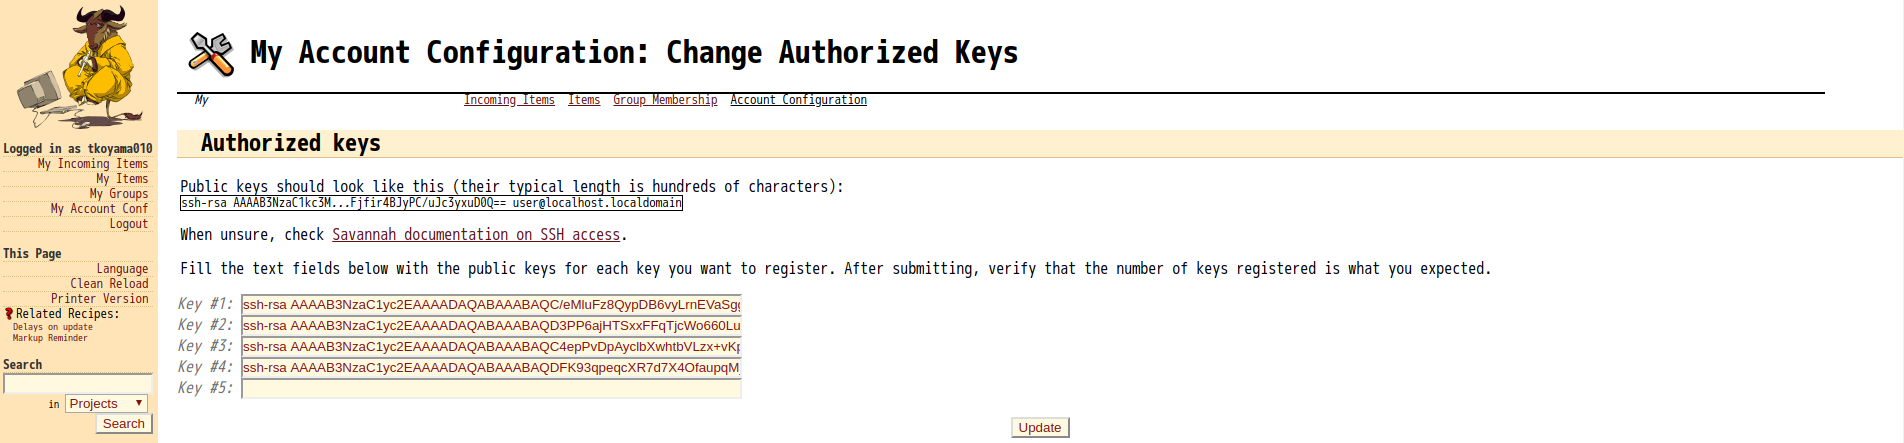
\includegraphics[width=1.0\textwidth]{fig/savannah-authorized-keys.eps}
\caption{\href{https://savannah.gnu.org/my/admin/editsshkeys.php}{Savannahの承認鍵の設定}}
\label{fig:savannah-authorized-keys}
\end{figure}

\href{http://getfem.org}{GetFEM++}プロジェクトでソースの変更を行う際にはGitで以下のようにブランチを作成する規約となっています。
\begin{shbox}
  \shuser{developer}
  \shline{}{cd /path/to/getfem}
  \shline{}{git branch devel-name-subject}
  \shline{}{git checkout devel-name-subject}
\end{shbox}
ここで、\texttt{name}は開発者の名前、\texttt{subject}は開発内容としてください。
\footnote{
プロジェクトへの貢献方法はプログラムの新機能のパッチ作成だけではありません。
ドキュメントを読んでいる際に気づいたTypo(打ち間違い)の修正も大切な貢献です。
著者はTypoの修正のために\texttt{fixfixmisspell}という\texttt{branch}を作成したころ、Typo修正用の公式ブランチとして採用されました。
詳細は、 \href{http://getfem.org/project/contribute.html}{http://getfem.org/project/contribute.html} の"Specific branch for doc improvements and typo-fixes"を参照してください。
自分の小さな提案が採用されることもOSSへの貢献の面白さかと思います。
}
修正後コミットをしてブランチに\texttt{push}します。
\begin{shbox}
  \shuser{developer}
  \shline{}{cd /path/to/getfem}
  \shline{}{git commit -m"開発内容のメッセージ。もちろん英語!"}
  \shline{}{git push origin devel-name-subject}
\end{shbox}
修正後メーリングリスト\texttt{getfem-commits@nongnu.org}に連絡をして\texttt{master}ブランチへのマージを管理者にリクエストしてください。
\emph{誤って}\texttt{master}\emph{ブランチに}\texttt{push}\emph{しないように十分注意してください}!!!
管理者から注意されて\texttt{revert}されるでしょう。

\section{\href{http://getfem.org}{GetFEM++}のコンパイルとテスト方法}
\href{http://getfem.org}{GetFEM++}のコンパイルとテスト方法について説明します。
まずは、\texttt{getfem}のリポジトリ直下にある\texttt{autogen.sh}を実行します。
実行には\texttt{libtoolize}と\texttt{automake}が必要になりますので先にインストールしてください。
\begin{shbox}
  \shuser{devlname}
  \shline{} {sudo aptitude install libtool automake}
\end{shbox}
また、コンパイルに使用するライブラリとして以下のパッケージをインストールします。
\begin{itemize}
  \item \texttt{libqhull-dev} - calculate convex hulls and related structures (development files)
  \item \texttt{libmumps-dev} - Direct linear systems solver - parallel development files                  
  \item \texttt{libmumps-ptscotch-dev} - Direct linear systems solver - PTScotch-version development files          
  \item \texttt{libmumps-scotch-dev} - Direct linear systems solver - Scotch-version development files            
  \item \texttt{libmumps-seq-dev} - Direct linear systems solver - non-parallel development files              
  \item \texttt{liblapack-dev} - Library of linear algebra routines 3 - static version
  \item \texttt{libopenblas-dev} - Optimized BLAS (linear algebra) library (development files)
  \footnote{
    第14回オープンCAE勉強会@関東(構造など)にて\texttt{openblas}を使用すると通常の\texttt{blas}より高速になるとの指摘を\href{https://twitter.com/michioga}{@michioga}氏よりいただきました。
  }
\end{itemize}
さらに、\href{https://www.python.org/}{Python}のためのヘッダーファイルとスタテックライブラリScipyをインストールします。
\href{https://www.python.org/}{Python}2の場合
\begin{itemize}
  \item \texttt{python-dev} - header files and a static library for Python (default)
  \item \texttt{python-scipy} - scientific tools for Python
\end{itemize}
\href{https://www.python.org/}{Python}3の場合
\begin{itemize}
  \item \texttt{python3-dev} - header files and a static library for Python (default)
  \item \texttt{python3-scipy} - scientific tools for Python
\end{itemize}
をそれぞれインストールしてください。
インストール後\texttt{./configure}をプロジェクトフォルダで実行して、Makefileを作成します。
\href{https://www.python.org/}{Python}2の場合、
\begin{shbox}
  \shuser{developer}
  \shline{}{./configure --with-pic}
\end{shbox}
\href{https://www.python.org/}{Python}3の場合、
\begin{shbox}
  \shuser{developer}
  \shline{}{./configure --with-pic --enable-python3}
\end{shbox}
を実行します。
Makefile作成後以下のコマンドでコンパイルとテストの実行をします。
\begin{shbox}
  \shuser{developer}
  \shline{}{make \&\& make check}
\end{shbox}
\href{https://www.gnu.org/software/automake/}{\texttt{automake}}により整備されたテスト項目が実行され結果がログファイル\texttt{tests/test-suite.log}に出力されます。
テストに失敗した場合は\texttt{getfem-users@nongnu.org}に\texttt{tests/test-suite.log}を添付し報告をしてください(\emph{もちろんメッセージは英語で}!!!)。

\section{\href{http://www.sphinx-doc.org/ja/stable/intl.html}{GetFEM++のSphinxドキュメント日本語化プロジェクト}}
\subsection{\href{https://pypi.org/project/sphinx-intl/}{\texttt{sphinx-intl}}による翻訳ワークフロー}
\href{http://getfem.org}{GetFEM++}の\href{http://www.sphinx-doc.org/ja/stable/}{Sphinx}ドキュメントをコンパイルするには\texttt{doc}/\texttt{sphinx}で以下のコマンドを実行します。
\begin{shbox}
  \shuser{translator}
  \shline{}{make html (htmlを作成する場合)}
  \shline{}{make pdf  (pdfを作成する場合)}
\end{shbox}
これにより\texttt{doc}/\texttt{sphinx}/\texttt{build}以下の\texttt{html}ディレクトリと\texttt{pdf}ディレクトリにドキュメントが作成されます。
コンパイルされた\href{http://www.sphinx-doc.org/ja/stable/}{Sphinx}ドキュメントを
\href{http://www.sphinx-doc.org/ja/stable/intl.html}{国際化}のページを元に翻訳します。
ワークフローを\autoref{fig:translation}に示します。
一連の作業は\href{https://pypi.org/project/sphinx-intl/}{sphinx-intl}を使用して行います。
\href{https://pypi.org/project/sphinx-intl/}{sphinx-intl}は\href{http://www.sphinx-doc.org/ja/stable/}{Sphinx}での翻訳フローを便利にするツールです。
\begin{figure}[htbp]
\centering
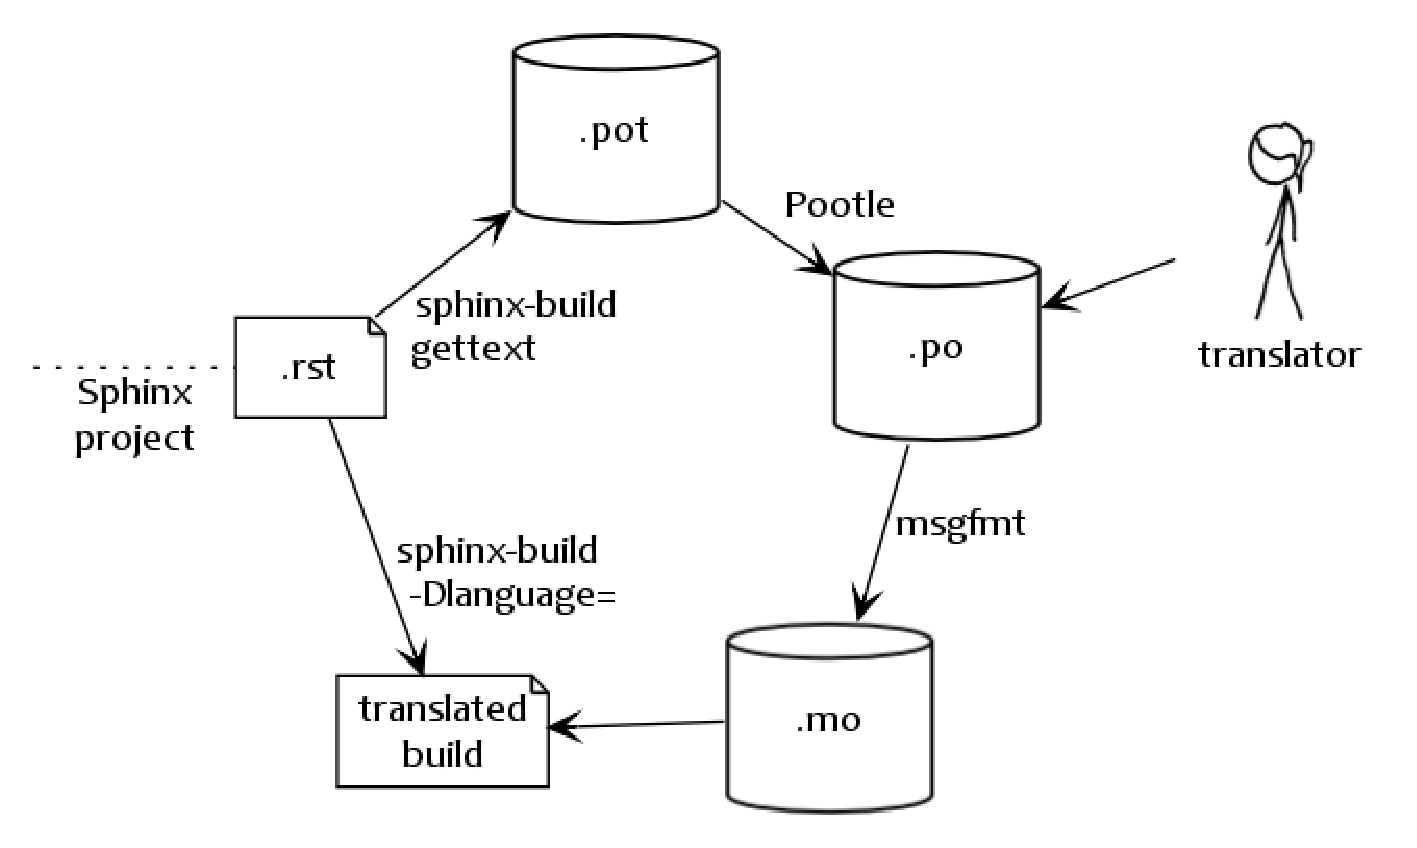
\includegraphics[width=0.5\textwidth]{fig/translation.eps}
\caption{\href{http://www.sphinx-doc.org/ja/stable/_images/translation.png}{Sphinxによる翻訳のビジュアルなワークフロー}
(\href{http://www.sphinx-doc.org/ja/stable/intl.html}{「国際化」}より引用)}
\label{fig:translation}
\end{figure}
\texttt{sphinx-intl}のインストールは\texttt{pip}を使用して以下のように行います。
\begin{shbox}
  \shuser{translator}
  \shline{}{sudo aptitude install python-pip}
  \shline{}{sudo pip install sphinx-intl}
\end{shbox}
\texttt{aptitude}で\texttt{sphinx-intl}をインストールをすることも可能ですが、\href{https://www.python.org/}{Python}2のバージョンを確実にイントールするためにこの方法をとります。
次に、\texttt{doc/sphinx/Makefile.am}と\texttt{doc/sphinx/source/conf.py}に以下の変更を適用します
(\texttt{「\href{http://www.turbare.net/weblog/workflow-with-transifex-and-sphinx.html}{Sphinx と transifex を活用した翻訳手順}」(Oct.14,2018 05:45 UTC)を参照})。
\footnote{
変更は2018年10月14日現在はブランチ\texttt{devel-tetsuo-translation}にコミットされています。
コミットのSHA-1ハッシュは\texttt{d3d1d625c62e3e974087a7c16e2d13ed294c576d}です。
管理者の承認が得られた場合\texttt{master}にマージされます。
}
\begin{lstlisting}[language=diff]
diff --git a/doc/sphinx/Makefile.am b/doc/sphinx/Makefile.am
index adb8259e..2cab2a69 100644
--- a/doc/sphinx/Makefile.am
+++ b/doc/sphinx/Makefile.am
@@ -21,8 +21,10 @@
 # You can set these variables from the command line.
 PYTHON        = python
 SPHINXROOT    = http://svn.python.org/projects
-SPHINXOPTS    =
+LANGUAGE      = en
+SPHINXOPTS    = -D language=$(LANGUAGE)
 SPHINXBUILD   = $(PYTHON) tools/sphinx-build.py
+SPHINXINTL    = sphinx-intl
 PAPER         =
 SOURCES       = $(srcdir)/source
 DISTVERSION   = @VERSION@
@@ -33,8 +35,9 @@ PAPEROPT_a4     = -D latex_paper_size=a4
 PAPEROPT_letter = -D latex_paper_size=letter
 ALLSPHINXOPTS   = -b $(BUILDER) -d build/doctrees $(PAPEROPT_$(PAPER)) \
                   $(SPHINXOPTS) $(SOURCES) build/$(BUILDER)
+I18NSPHINXOPTS  = $(SPHINXOPTS) ./source

-.PHONY: help checkout update images build view html htmlview htmlhelp latex pdf linkcheck clean upload
+.PHONY: help checkout update images build view html htmlview htmlhelp latex pdf linkcheck clean upload gettext


 help:
@@ -85,6 +88,7 @@ images:
        -cd $(srcdir)/source/scilab/images/; make png

 build: $(srcdir)/source/matlab/cmdref.rst $(srcdir)/source/python/cmdref.rst $(srcdir)/source/scilab/cmdref.rst checkout images
+       $(SPHINXINTL) build
        echo # rm -fr build/$(BUILDER)/_images
        echo # rm -fr build/$(BUILDER)/*.png
        mkdir -p build/$(BUILDER) build/doctrees
@@ -110,7 +114,7 @@ htmlhelp: build
 latex: BUILDER = latex
 latex: build
        @echo "Build finished; the LaTeX files are in build/latex."
-       @echo "Run \`make all-pdf' or \`make all-ps' in that directory to" \
+       @echo "Run \`make all-pdf' in that directory to" \
              "run these through (pdf)latex."

 pdf: BUILDER = latex
@@ -122,6 +126,11 @@ linkcheck: BUILDER = linkcheck
 linkcheck: build
        @echo "Link check complete; look for any errors in the above output " \
              "or in build/$(BUILDER)/output.txt."
+gettext:
+       $(SPHINXBUILD) -b gettext $(I18NSPHINXOPTS) locale
+       $(SPHINXINTL) update -p locale -l $(LANGUAGE)
+       @echo
+       @echo "Build finished. The message catalogs are in locale."

 clean:
        -rm -rf build/
\end{lstlisting}
\begin{lstlisting}[language=diff]
diff --git a/doc/sphinx/source/conf.py b/doc/sphinx/source/conf.py
index 14377f9d..fcaf2b7c 100644
--- a/doc/sphinx/source/conf.py
+++ b/doc/sphinx/source/conf.py
@@ -55,7 +55,7 @@ extensions = ['sphinx.ext.pngmath','sphinx.ext.autodoc',
 #source_suffix = '.rst'

 # The encoding of source files.
-#source_encoding = 'utf-8'
+source_encoding = 'utf-8'

 # The master toctree document.
 #master_doc = 'contents'
@@ -75,6 +75,9 @@ extensions = ['sphinx.ext.pngmath','sphinx.ext.autodoc',
 # relative to the source directory
 #locale_dirs = []

+gettext_compact = False
+locale_dirs = ['locale/']
+
 # Add any paths that contain templates here, relative to this directory.
 templates_path = ['.templates']
\end{lstlisting}
つぎに、以下のコマンドを\texttt{doc/sphinx}以下で実行し\texttt{locale}ディレクトリ以下を初期設定あるいは更新をします。
\begin{shbox}
  \shuser{translator}
  \shline{}{make gettext}
\end{shbox}
このコマンドを実行すると\texttt{pot}ファイルの作成と、
\texttt{./locale/ja/LC_MESSAGES/}以下に\texttt{po}のファイルが作成もしくは更新されます。
\autoref{fig:translation}に示すように翻訳者は\texttt{po}ファイルの中身を編集します。
\texttt{po}ファイルの中身は次のようになっています。
\begin{lstlisting}[language=]
#: src/name.c:36
msgid "My name is %s.\n"
msgstr ""
\end{lstlisting}
翻訳者はこのファイルを編集し以下のようにします。(\texttt{「\href{https://ja.wikipedia.org/wiki/Gettext}{gettext - Wikipedia}」(Oct.13,2018 17:31 UTC) より引用})
\begin{lstlisting}[language=]
#: src/name.c:36
msgid "My name is %s.\n"
msgstr "私の名前は %sです。\n"
\end{lstlisting}
翻訳が完了したら、\texttt{make html}もしくは\texttt{make latex}コマンドを実行します。
\texttt{LANGUAGE}の\texttt{en}の部分は日本語の翻訳を適用する際には\texttt{ja}に変更してください。
翻訳を適用する場合は\texttt{make pdf}は使用できないため注意してください。
\texttt{make latex}を実行した後\texttt{doc/sphinx/build/latex}以下で\texttt{make all-pdf-ja}を実行してください。

\subsection{\href{https://www.transifex.com}{Transifex}の使用方法}
前節で作成した\texttt{*.po}ファイルを\href{https://www.transifex.com}{Transifex}を使用して管理します。
\href{https://www.transifex.com}{Transifex}のサービスについて\href{https://ja.wikipedia.org/wiki/Transifex}{Wikipedia}の内容を引用します。

\begin{quote}
\href{https://www.transifex.com}{Transifex}はWebベースの翻訳プラットフォームであり、ローカライズ管理システムとしても知られている。 
ソフトウェア、文書、Webサイトなど頻繁に更新されるコンテンツと技術的なプロジェクトを対象とし、開発者が使用するツールと統合することにより翻訳ワークフローを自動化している。
有料機能とオープンソースプロジェクト用の無料アカウント機能の両方をSaaSとして提供している。
サイト内では翻訳者が共同作業できるようにするために翻訳対象のファイルホスティングや、フィード、掲示板投稿、翻訳提案や投票などのソーシャル・ネットワーキング・サービスとしての機能が利用できる。
サイトはDjangoとPythonで構築されている。
\texttt{「\href{https://ja.wikipedia.org/wiki/Transifex}{Transifex - Wikipedia}」(Oct.14,2018 06:28 UTC) より引用}
\end{quote}
本プロジェクトで新しくGetFEM++5.3の翻訳プロジェクトのために\autoref{fig:transifex-getfem-5.3}のページを作成しました。
翻訳の提案などはこちらのページで行うことができます。
\begin{figure}[htbp]
\centering
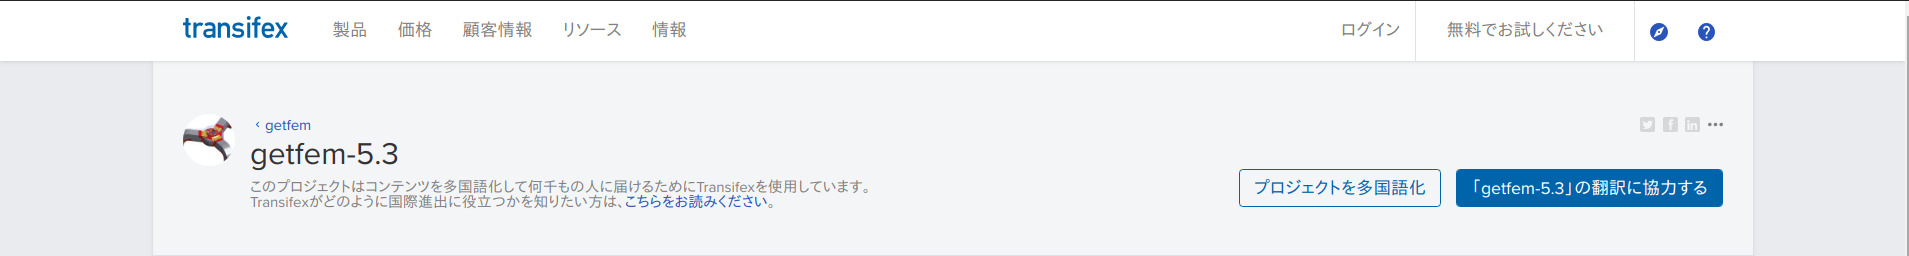
\includegraphics[width=1.0\textwidth]{fig/transifex-getfem-53.eps}
\caption{\href{https://www.transifex.com/getfem-doc/getfem-53-1/dashboard/}{GetFEM++5.3翻訳プロジェクト}}
\label{fig:transifex-getfem-5.3}
\end{figure}
\href{https://www.transifex.com}{Transifex}での翻訳結果を反映するためにはクライアントコマンド\texttt{tx}を使用します。
\texttt{tx}コマンドは以下のようにインストールします。
\begin{shbox}
  \shuser{translator}
  \shline{}{sudo aptitude install transifex-client}
\end{shbox}
インストール後\texttt{doc/sphinx}以下で以下のコマンドを実行してください。
\begin{shbox}
  \shline{}{tx pull -l ja}
\end{shbox}
このコマンドは設定ファイル\texttt{doc/sphinx/.tx/config}を参照して\texttt{source/locale}以下に\texttt{*.po}ファイルをダウンロードするコマンドです。
\footnote{
\texttt{doc/sphinx/.tx/config}はバージョンアップの際にTransifexのページ管理者が更新を行います。
\texttt{doc/sphinx}で以下のコマンドを実行します。
\begin{shbox}
  \shuser{admin}
  \shline{}{sphinx-intl update-txconfig-resources --pot-dir build/locale --transifex-project-name="getfem-<version number>"}
\end{shbox}
}
APIキーを聞かれた際には\href{https://www.transifex.com}{Transifex}のアカウントのページでAPIキーを発行してください。
\texttt{po}ファイルをダウンロード後、前節で紹介した手順で翻訳されたドキュメントを作成します。
なお本プロジェクトではトラブル防止のため、翻訳の修正を提案する場合は必ず\href{https://www.transifex.com}{Transifex}のWebページから行ってください。
\texttt{tx push}コマンドは使用しないでください。
また、\texttt{tx push}をした後に\texttt{make gettext}を行うと\texttt{po}ファイルが更新されダウンロードした翻訳が消えることがあるため注意してください。

\section{技術書典5サークル参加}
翻訳した文書を頒布するため、技術書の即売会である\href{https://techbookfest.org/event/tbf05}{技術書典5}に参加しました。
出典ブースの様子を\autoref{fig:tecbookfest5-boose}に示します。
日時は 2018/10/08 (月) 11:00〜17:00 で場所は 池袋サンシャインシティ2F 展示ホールD(文化会館ビル2F) でした。
50部を印刷し、頒布数は38部(内4部は挨拶用・2部はオープンCAE勉強会参加者様)でした。
%
\begin{figure}[htbp]
\centering
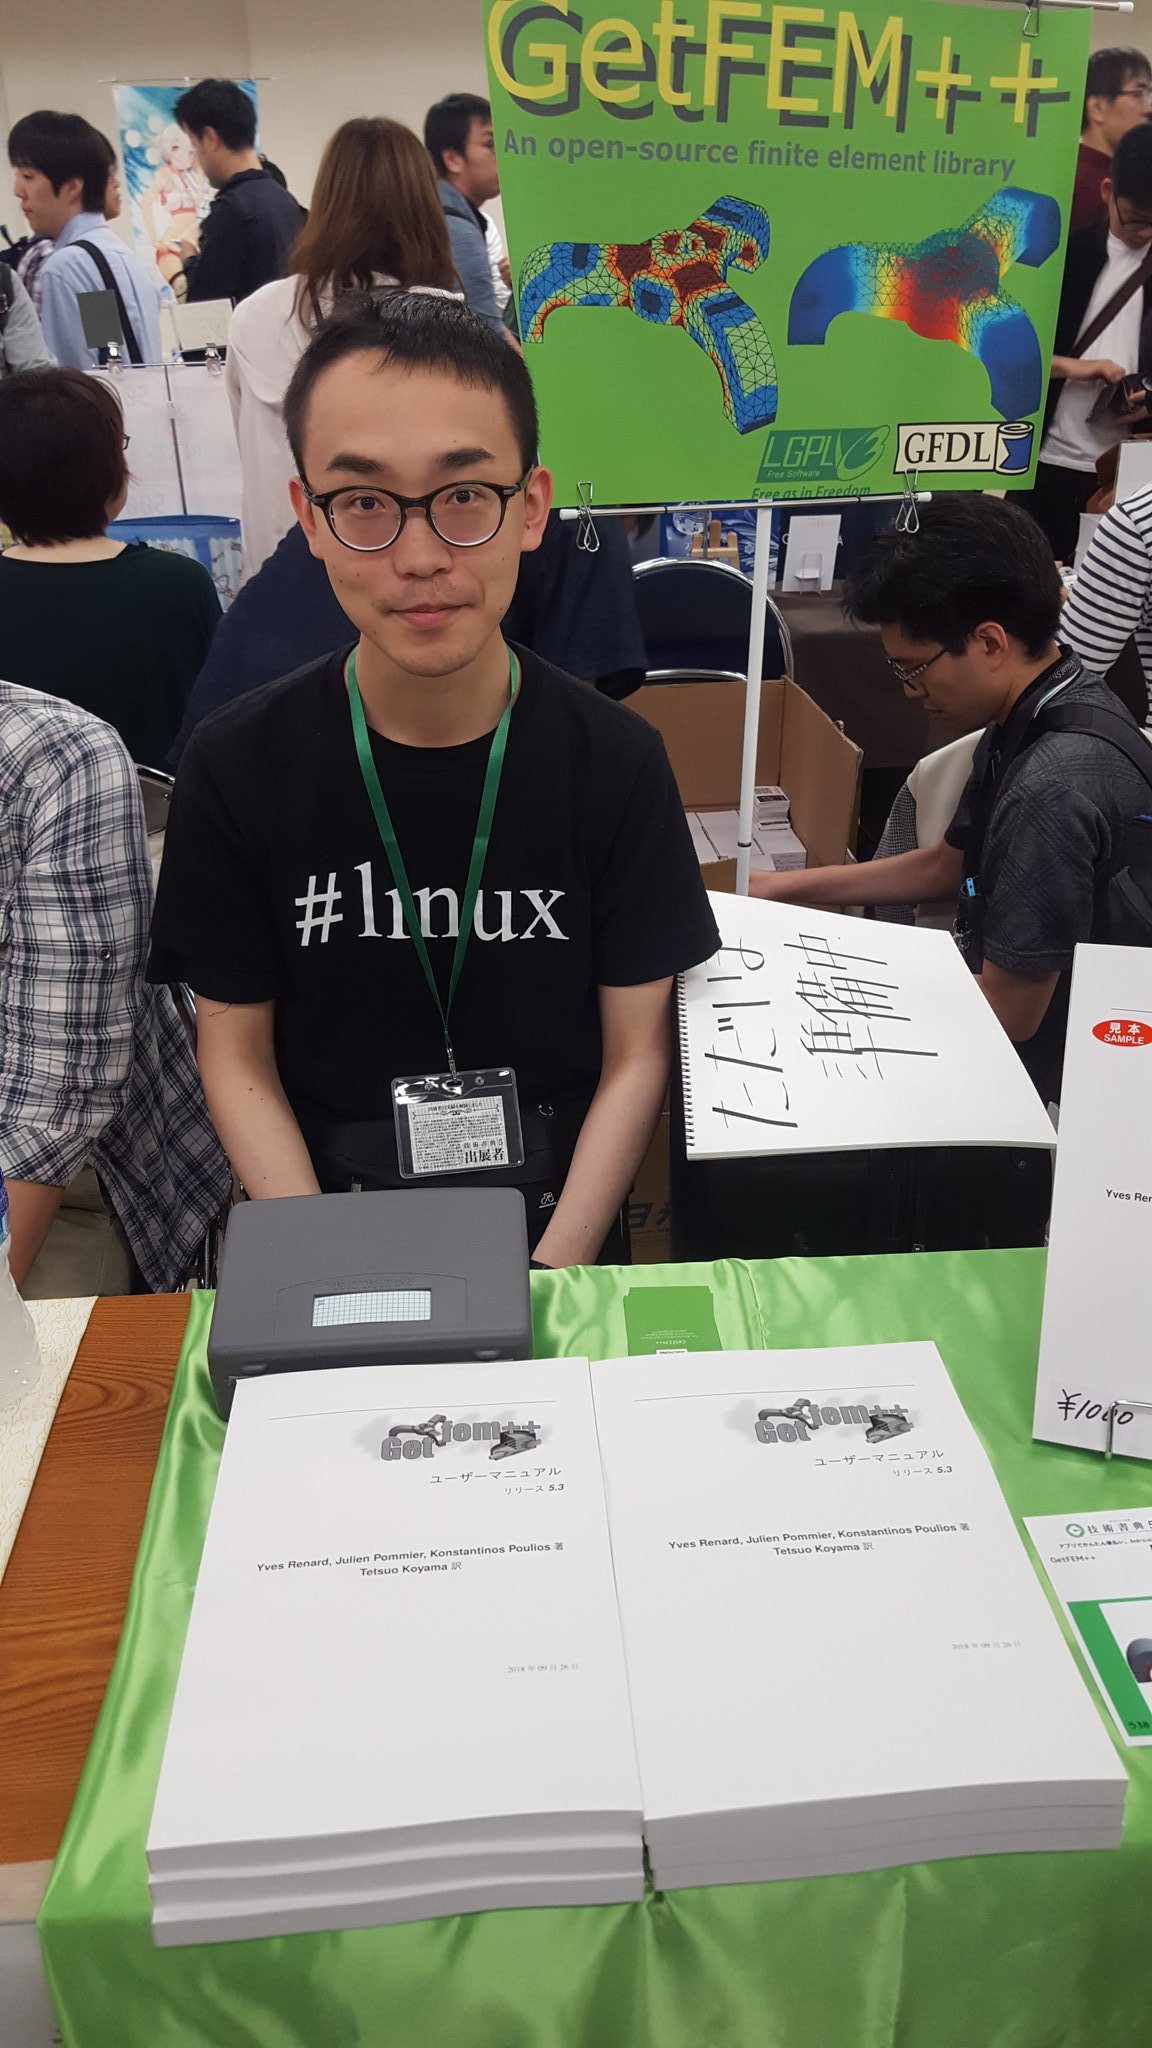
\includegraphics[width=0.25\textwidth]{fig/boose-1.eps}
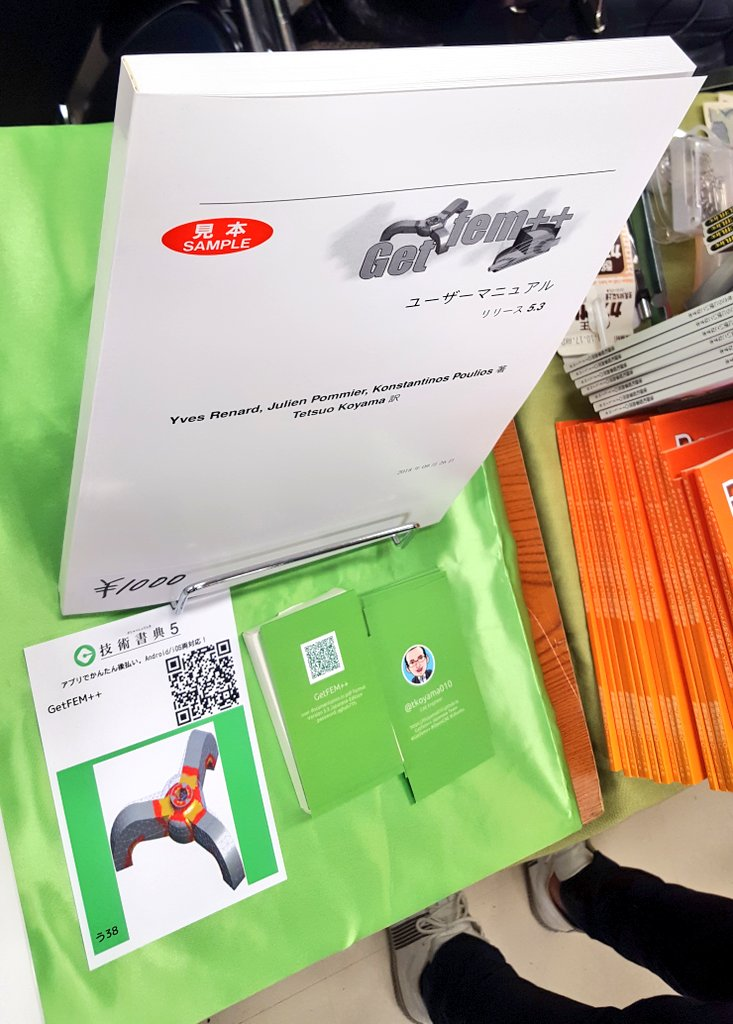
\includegraphics[width=0.25\textwidth]{fig/boose-2.eps}
\caption{\href{https://techbookfest.org/event/tbf05}{サークルGetFEM++@技術書典5のブース}}
\label{fig:tecbookfest5-boose}
\end{figure}
ブースには以下の方ような方がいらっしゃいました。
\begin{itemize}
  \item{昔商用FEMコードを使われていて今は使われていない方}
  \item{商用FEMコードを使用されている方}
  \item{これからFEMを勉強される学生の方}
  \item{OpenFOAMを使用されていて、構造にもオープンソースがあることをはじめて知った方}
  \item{ポスターの絵がきっかけでCAEに興味を持たれた方}
\end{itemize}
一般購入者の方で構造でオープンソースを使用されている方はおらず、ポスターのような解析がオープンソースでもできることに驚かれもしました。
オープンソースの有限要素法解析ソフトへの認知度は低く、今後も認知のためのドキュメント頒布が必要と考えています。
次回の出典では\autoref{fig:tecbookfest6-book}に示す3冊のドキュメントの配布を予定しています。
%
\begin{figure}[htbp]
\centering
\fbox{
\includegraphics[width=0.250\textwidth]{fig/getfem-project-face.eps}}
\fbox{
\includegraphics[width=0.255\textwidth]{fig/getfem-tutorial-face.eps}}
\fbox{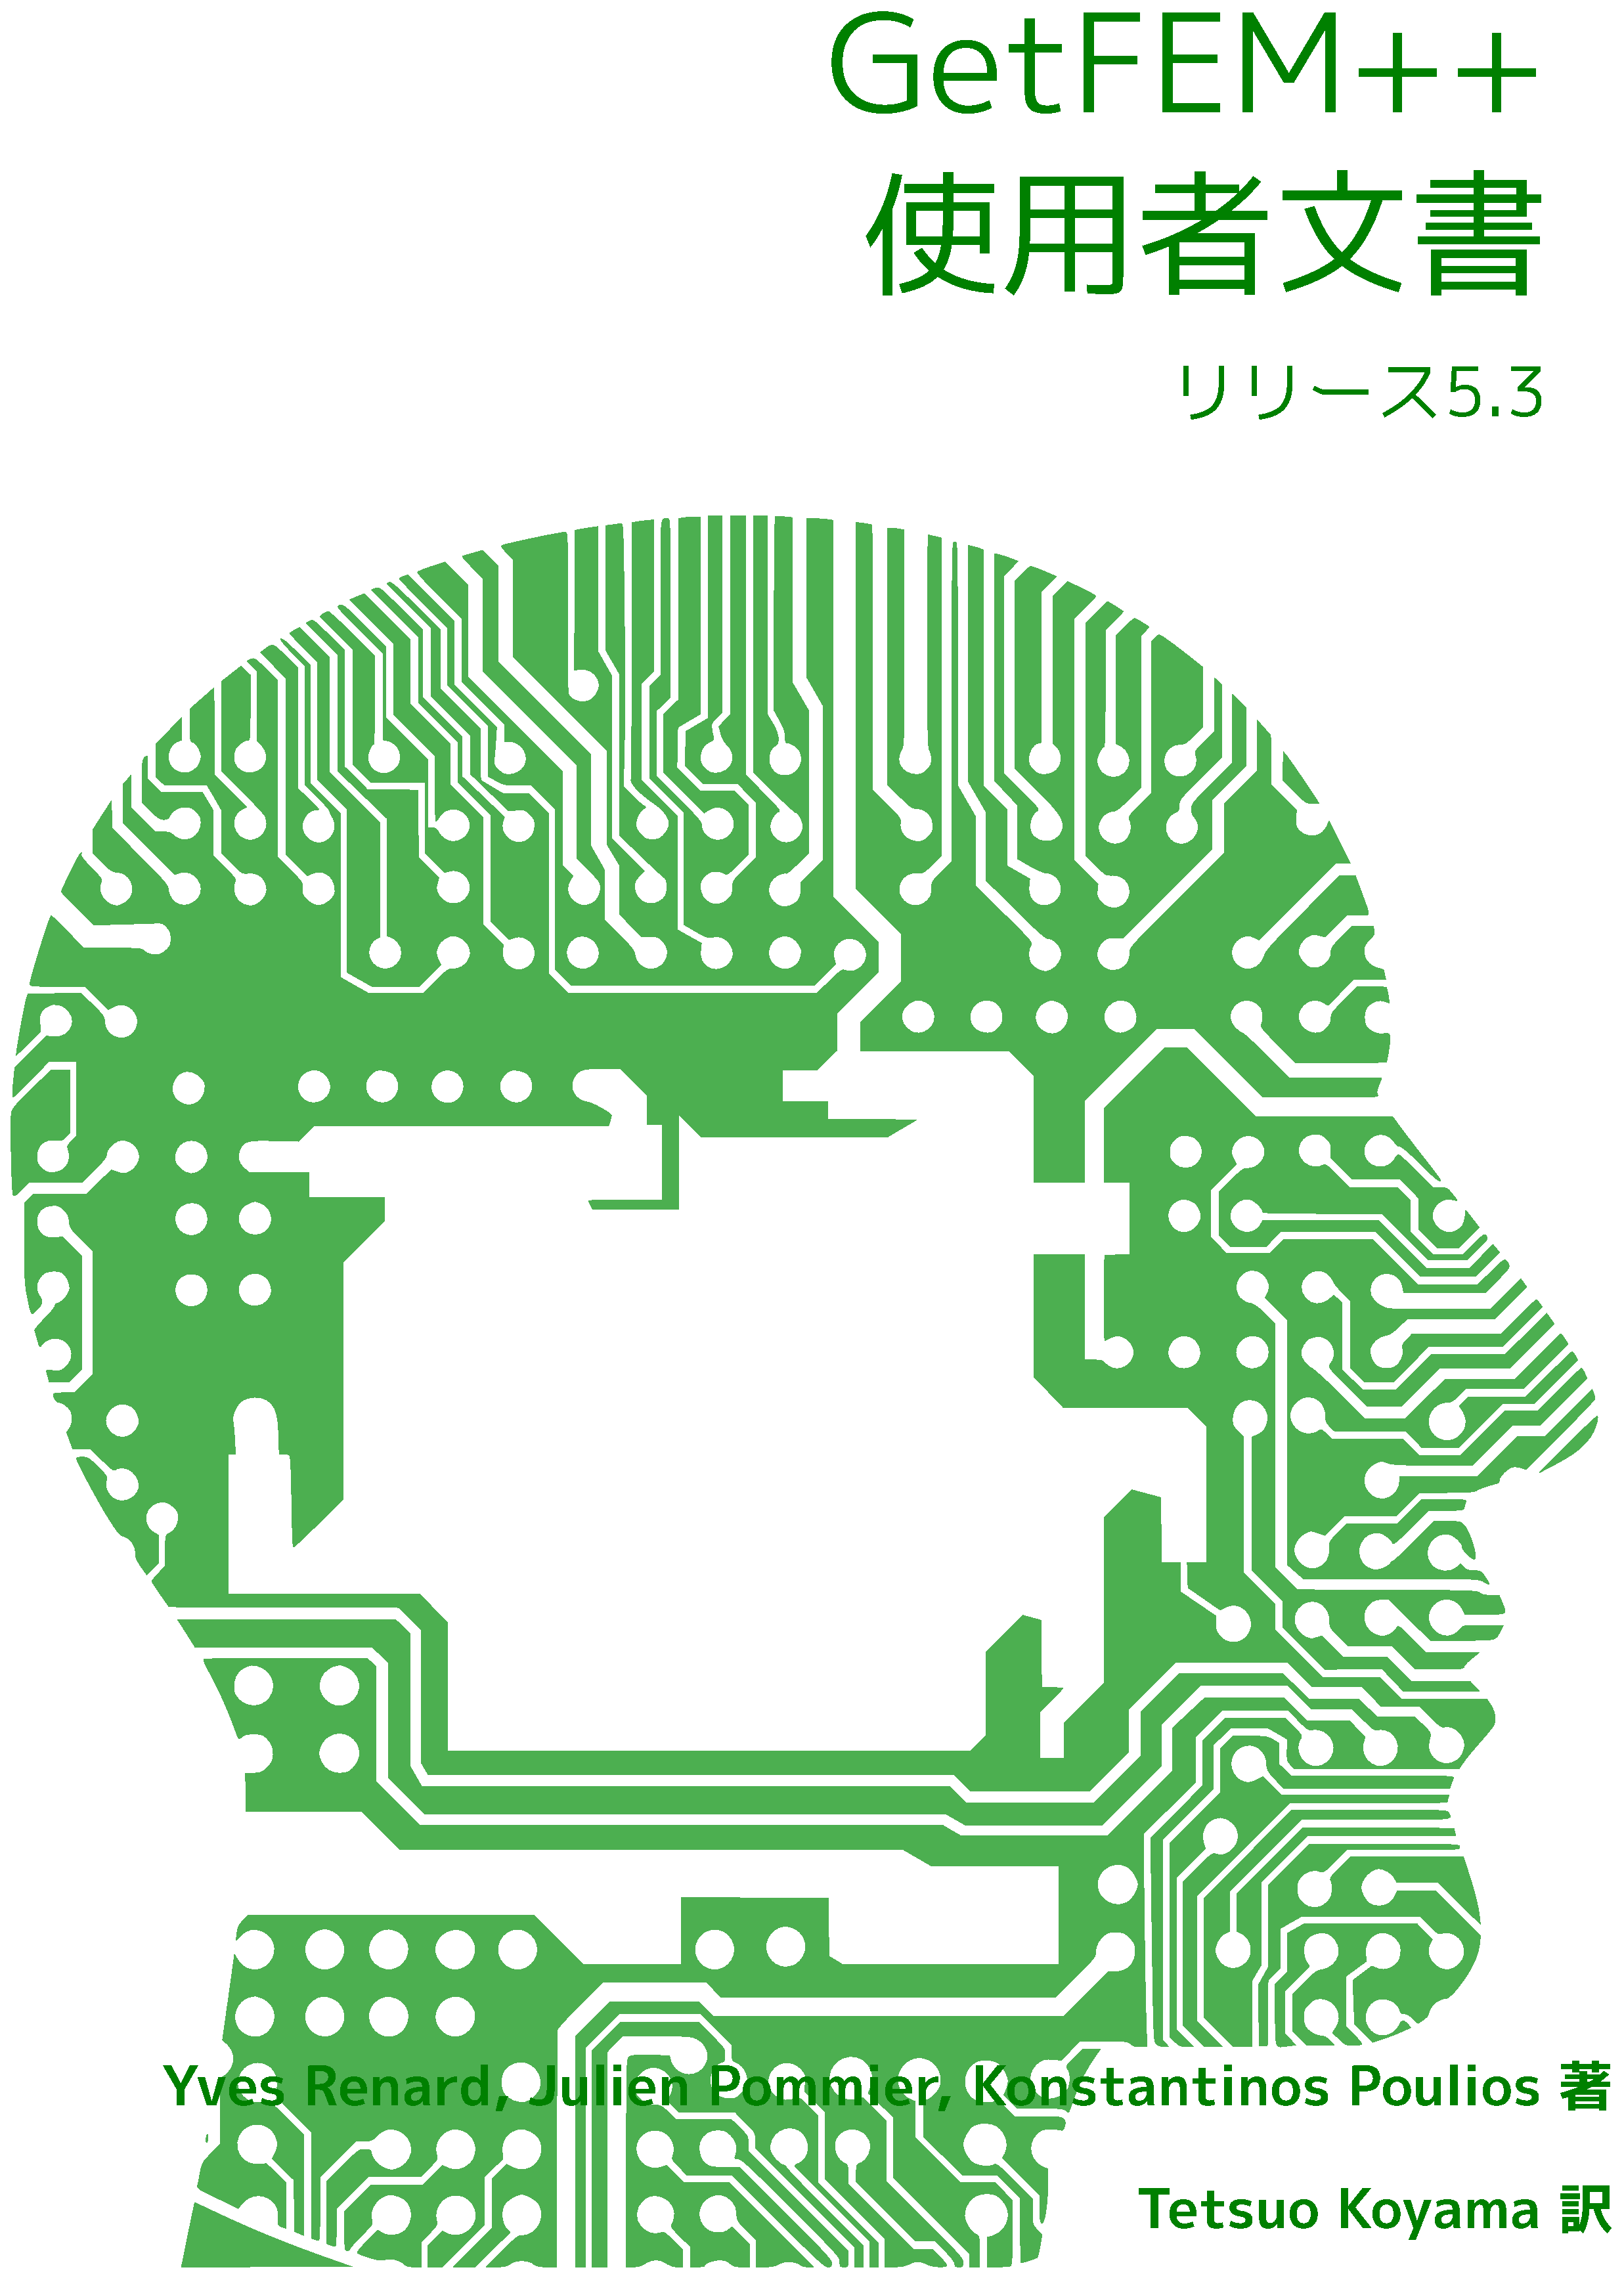
\includegraphics[width=0.250\textwidth]{fig/getfem-userdoc-face.eps}}
\caption{\href{https://techbookfest.org}{次回配布予定のドキュメント}}
\label{fig:tecbookfest6-book}
\end{figure}
\section{まとめ}
\begin{itemize}
  \item{\href{https://ja.wikipedia.org/wiki/GetFEM++}{GetFEM++のWikipediaの日本語版}を作成することによりGetFEM++プロジェクトの目的を紹介した。}
  \item{\href{http://getfem.org}{GetFEM++}のソースのホスティングサービス\href{https://savannah.gnu.org}{Savannah}でプロジェクトに貢献する方法を紹介した。}
  \item{\href{http://www.sphinx-doc.org/ja/stable/intl.html}{GetFEM++のSphinxドキュメント日本語化プロジェクト}の内容について紹介した。}
  \item{\href{https://techbookfest.org/event/tbf05}{技術書典5}への参加報告をおこなった。}
\end{itemize}
\appendix
\section{translate-shellの使用方法}
執筆中
\section{GithubPagesでの公開}
執筆中
\end{document}
